% Modified for NDSS 2024 by MS on 2024/07/01

%% bare_conf.tex
%% V1.4b
%% 2015/08/26
%% by Michael Shell
%% See:
%% http://www.michaelshell.org/
%% for current contact information.
%%
%% This is a skeleton file demonstrating the use of IEEEtran.cls
%% (requires IEEEtran.cls version 1.8b or later) with an IEEE
%% conference paper.
%%
%% Support sites:
%% http://www.michaelshell.org/tex/ieeetran/
%% http://www.ctan.org/pkg/ieeetran
%% and
%% http://www.ieee.org/

%%*************************************************************************
%% Legal Notice:
%% This code is offered as-is without any warranty either expressed or
%% implied; without even the implied warranty of MERCHANTABILITY or
%% FITNESS FOR A PARTICULAR PURPOSE! 
%% User assumes all risk.
%% In no event shall the IEEE or any contributor to this code be liable for
%% any damages or losses, including, but not limited to, incidental,
%% consequential, or any other damages, resulting from the use or misuse
%% of any information contained here.
%%
%% All comments are the opinions of their respective authors and are not
%% necessarily endorsed by the IEEE.
%%
%% This work is distributed under the LaTeX Project Public License (LPPL)
%% ( http://www.latex-project.org/ ) version 1.3, and may be freely used,
%% distributed and modified. A copy of the LPPL, version 1.3, is included
%% in the base LaTeX documentation of all distributions of LaTeX released
%% 2003/12/01 or later.
%% Retain all contribution notices and credits.
%% ** Modified files should be clearly indicated as such, including  **
%% ** renaming them and changing author support contact information. **
%%*************************************************************************


% *** Authors should verify (and, if needed, correct) their LaTeX system  ***
% *** with the testflow diagnostic prior to trusting their LaTeX platform ***
% *** with production work. The IEEE's font choices and paper sizes can   ***
% *** trigger bugs that do not appear when using other class files.       ***                          ***
% The testflow support page is at:
% http://www.michaelshell.org/tex/testflow/



\documentclass[conference]{IEEEtran}
% --- Added for NDSS poster submission (figures/URLs) ---
\usepackage{graphicx}
\usepackage{url}
% Some Computer Society conferences also require the compsoc mode option,
% but others use the standard conference format.
%
% If IEEEtran.cls has not been installed into the LaTeX system files,
% manually specify the path to it like:
% \documentclass[conference]{../sty/IEEEtran}





% Some very useful LaTeX packages include:
% (uncomment the ones you want to load)


% *** MISC UTILITY PACKAGES ***
%
%\usepackage{ifpdf}
% Heiko Oberdiek's ifpdf.sty is very useful if you need conditional
% compilation based on whether the output is pdf or dvi.
% usage:
% \ifpdf
%   % pdf code
% \else
%   % dvi code
% \fi
% The latest version of ifpdf.sty can be obtained from:
% http://www.ctan.org/pkg/ifpdf
% Also, note that IEEEtran.cls V1.7 and later provides a builtin
% \ifCLASSINFOpdf conditional that works the same way.
% When switching from latex to pdflatex and vice-versa, the compiler may
% have to be run twice to clear warning/error messages.






% *** CITATION PACKAGES ***
%
%\usepackage{cite}
% cite.sty was written by Donald Arseneau
% V1.6 and later of IEEEtran pre-defines the format of the cite.sty package
% \cite{} output to follow that of the IEEE. Loading the cite package will
% result in citation numbers being automatically sorted and properly
% "compressed/ranged". e.g., [1], [9], [2], [7], [5], [6] without using
% cite.sty will become [1], [2], [5]--[7], [9] using cite.sty. cite.sty's
% \cite will automatically add leading space, if needed. Use cite.sty's
% noadjust option (cite.sty V3.8 and later) if you want to turn this off
% such as if a citation ever needs to be enclosed in parenthesis.
% cite.sty is already installed on most LaTeX systems. Be sure and use
% version 5.0 (2009-03-20) and later if using hyperref.sty.
% The latest version can be obtained at:
% http://www.ctan.org/pkg/cite
% The documentation is contained in the cite.sty file itself.






% *** GRAPHICS RELATED PACKAGES ***
%
\ifCLASSINFOpdf
  % \usepackage[pdftex]{graphicx}
  % declare the path(s) where your graphic files are
  % \graphicspath{{../pdf/}{../jpeg/}}
  % and their extensions so you won't have to specify these with
  % every instance of \includegraphics
  % \DeclareGraphicsExtensions{.pdf,.jpeg,.png}
\else
  % or other class option (dvipsone, dvipdf, if not using dvips). graphicx
  % will default to the driver specified in the system graphics.cfg if no
  % driver is specified.
  % \usepackage[dvips]{graphicx}
  % declare the path(s) where your graphic files are
  % \graphicspath{{../eps/}}
  % and their extensions so you won't have to specify these with
  % every instance of \includegraphics
  % \DeclareGraphicsExtensions{.eps}
\fi
% graphicx was written by David Carlisle and Sebastian Rahtz. It is
% required if you want graphics, photos, etc. graphicx.sty is already
% installed on most LaTeX systems. The latest version and documentation
% can be obtained at: 
% http://www.ctan.org/pkg/graphicx
% Another good source of documentation is "Using Imported Graphics in
% LaTeX2e" by Keith Reckdahl which can be found at:
% http://www.ctan.org/pkg/epslatex
%
% latex, and pdflatex in dvi mode, support graphics in encapsulated
% postscript (.eps) format. pdflatex in pdf mode supports graphics
% in .pdf, .jpeg, .png and .mps (metapost) formats. Users should ensure
% that all non-photo figures use a vector format (.eps, .pdf, .mps) and
% not a bitmapped formats (.jpeg, .png). The IEEE frowns on bitmapped formats
% which can result in "jaggedy"/blurry rendering of lines and letters as
% well as large increases in file sizes.
%
% You can find documentation about the pdfTeX application at:
% http://www.tug.org/applications/pdftex





% *** MATH PACKAGES ***
%
%\usepackage{amsmath}
% A popular package from the American Mathematical Society that provides
% many useful and powerful commands for dealing with mathematics.
%
% Note that the amsmath package sets \interdisplaylinepenalty to 10000
% thus preventing page breaks from occurring within multiline equations. Use:
%\interdisplaylinepenalty=2500
% after loading amsmath to restore such page breaks as IEEEtran.cls normally
% does. amsmath.sty is already installed on most LaTeX systems. The latest
% version and documentation can be obtained at:
% http://www.ctan.org/pkg/amsmath





% *** SPECIALIZED LIST PACKAGES ***
%
%\usepackage{algorithmic}
% algorithmic.sty was written by Peter Williams and Rogerio Brito.
% This package provides an algorithmic environment fo describing algorithms.
% You can use the algorithmic environment in-text or within a figure
% environment to provide for a floating algorithm. Do NOT use the algorithm
% floating environment provided by algorithm.sty (by the same authors) or
% algorithm2e.sty (by Christophe Fiorio) as the IEEE does not use dedicated
% algorithm float types and packages that provide these will not provide
% correct IEEE style captions. The latest version and documentation of
% algorithmic.sty can be obtained at:
% http://www.ctan.org/pkg/algorithms
% Also of interest may be the (relatively newer and more customizable)
% algorithmicx.sty package by Szasz Janos:
% http://www.ctan.org/pkg/algorithmicx




% *** ALIGNMENT PACKAGES ***
%
%\usepackage{array}
% Frank Mittelbach's and David Carlisle's array.sty patches and improves
% the standard LaTeX2e array and tabular environments to provide better
% appearance and additional user controls. As the default LaTeX2e table
% generation code is lacking to the point of almost being broken with
% respect to the quality of the end results, all users are strongly
% advised to use an enhanced (at the very least that provided by array.sty)
% set of table tools. array.sty is already installed on most systems. The
% latest version and documentation can be obtained at:
% http://www.ctan.org/pkg/array


% IEEEtran contains the IEEEeqnarray family of commands that can be used to
% generate multiline equations as well as matrices, tables, etc., of high
% quality.




% *** SUBFIGURE PACKAGES ***
%\ifCLASSOPTIONcompsoc
%  \usepackage[caption=false,font=normalsize,labelfont=sf,textfont=sf]{subfig}
%\else
%  \usepackage[caption=false,font=footnotesize]{subfig}
%\fi
% subfig.sty, written by Steven Douglas Cochran, is the modern replacement
% for subfigure.sty, the latter of which is no longer maintained and is
% incompatible with some LaTeX packages including fixltx2e. However,
% subfig.sty requires and automatically loads Axel Sommerfeldt's caption.sty
% which will override IEEEtran.cls' handling of captions and this will result
% in non-IEEE style figure/table captions. To prevent this problem, be sure
% and invoke subfig.sty's "caption=false" package option (available since
% subfig.sty version 1.3, 2005/06/28) as this is will preserve IEEEtran.cls
% handling of captions.
% Note that the Computer Society format requires a larger sans serif font
% than the serif footnote size font used in traditional IEEE formatting
% and thus the need to invoke different subfig.sty package options depending
% on whether compsoc mode has been enabled.
%
% The latest version and documentation of subfig.sty can be obtained at:
% http://www.ctan.org/pkg/subfig




% *** FLOAT PACKAGES ***
%
%\usepackage{fixltx2e}
% fixltx2e, the successor to the earlier fix2col.sty, was written by
% Frank Mittelbach and David Carlisle. This package corrects a few problems
% in the LaTeX2e kernel, the most notable of which is that in current
% LaTeX2e releases, the ordering of single and double column floats is not
% guaranteed to be preserved. Thus, an unpatched LaTeX2e can allow a
% single column figure to be placed prior to an earlier double column
% figure.
% Be aware that LaTeX2e kernels dated 2015 and later have fixltx2e.sty's
% corrections already built into the system in which case a warning will
% be issued if an attempt is made to load fixltx2e.sty as it is no longer
% needed.
% The latest version and documentation can be found at:
% http://www.ctan.org/pkg/fixltx2e


%\usepackage{stfloats}
% stfloats.sty was written by Sigitas Tolusis. This package gives LaTeX2e
% the ability to do double column floats at the bottom of the page as well
% as the top. (e.g., "\begin{figure*}[!b]" is not normally possible in
% LaTeX2e). It also provides a command:
%\fnbelowfloat
% to enable the placement of footnotes below bottom floats (the standard
% LaTeX2e kernel puts them above bottom floats). This is an invasive package
% which rewrites many portions of the LaTeX2e float routines. It may not work
% with other packages that modify the LaTeX2e float routines. The latest
% version and documentation can be obtained at:
% http://www.ctan.org/pkg/stfloats
% Do not use the stfloats baselinefloat ability as the IEEE does not allow
% \baselineskip to stretch. Authors submitting work to the IEEE should note
% that the IEEE rarely uses double column equations and that authors should try
% to avoid such use. Do not be tempted to use the cuted.sty or midfloat.sty
% packages (also by Sigitas Tolusis) as the IEEE does not format its papers in
% such ways.
% Do not attempt to use stfloats with fixltx2e as they are incompatible.
% Instead, use Morten Hogholm'a dblfloatfix which combines the features
% of both fixltx2e and stfloats:
%
% \usepackage{dblfloatfix}
% The latest version can be found at:
% http://www.ctan.org/pkg/dblfloatfix




% *** PDF, URL AND HYPERLINK PACKAGES ***
%
%\usepackage{url}
% url.sty was written by Donald Arseneau. It provides better support for
% handling and breaking URLs. url.sty is already installed on most LaTeX
% systems. The latest version and documentation can be obtained at:
% http://www.ctan.org/pkg/url
% Basically, \url{my_url_here}.




% *** Do not adjust lengths that control margins, column widths, etc. ***
% *** Do not use packages that alter fonts (such as pslatex).         ***
% There should be no need to do such things with IEEEtran.cls V1.6 and later.
% (Unless specifically asked to do so by the journal or conference you plan
% to submit to, of course. )


% correct bad hyphenation here
\hyphenation{op-tical net-works semi-conduc-tor}


\begin{document}
%
% paper title
% Titles are generally capitalized except for words such as a, an, and, as,
% at, but, by, for, in, nor, of, on, or, the, to and up, which are usually
% not capitalized unless they are the first or last word of the title.
% Linebreaks \\ can be used within to get better formatting as desired.
% Do not put math or special symbols in the title.
\title{Poster: GEM-PLI Side Channel in GPON\\ Inferring Encrypted Streaming Traffic}


% author names and affiliations
% use a multiple column layout for up to three different
% affiliations
\author{\IEEEauthorblockN{Hyunjun An}
	\IEEEauthorblockA{Heungdeok High School\\
		hjahn@anhyunjun.com}}
	
% conference papers do not typically use \thanks and this command
% is locked out in conference mode. If really needed, such as for
% the acknowledgment of grants, issue a \IEEEoverridecommandlockouts
% after \documentclass

% for over three affiliations, or if they all won't fit within the width
% of the page, use this alternative format:
% 
%\author{\IEEEauthorblockN{Michael Shell\IEEEauthorrefmark{1},
%Homer Simpson\IEEEauthorrefmark{2},
%James Kirk\IEEEauthorrefmark{3}, 
%Montgomery Scott\IEEEauthorrefmark{3} and
%Eldon Tyrell\IEEEauthorrefmark{4}}
%\IEEEauthorblockA{\IEEEauthorrefmark{1}School of Electrical and Computer Engineering\\
%Georgia Institute of Technology,
%Atlanta, Georgia 30332--0250\\ Email: see http://www.michaelshell.org/contact.html}
%\IEEEauthorblockA{\IEEEauthorrefmark{2}Twentieth Century Fox, Springfield, USA\\
%Email: homer@thesimpsons.com}
%\IEEEauthorblockA{\IEEEauthorrefmark{3}Starfleet Academy, San Francisco, California 96678-2391\\
%Telephone: (800) 555--1212, Fax: (888) 555--1212}
%\IEEEauthorblockA{\IEEEauthorrefmark{4}Tyrell Inc., 123 Replicant Street, Los Angeles, California 90210--4321}}




% use for special paper notices
%\IEEEspecialpapernotice{(Invited Paper)}


\IEEEoverridecommandlockouts
\makeatletter\def\@IEEEpubidpullup{6.5\baselineskip}\makeatother
\IEEEpubid{\parbox{\columnwidth}{
		Network and Distributed System Security (NDSS) Symposium 2026\\
		February 2026\\
		ISBN [TBD]\\
		https://dx.doi.org/10.14722/ndss.2026.[TBD]\\
		www.ndss-symposium.org
}
\hspace{\columnsep}\makebox[\columnwidth]{}}




% make the title area
\maketitle

% As a general rule, do not put math, special symbols or citations
% in the abstract
\begin{abstract}
Gigabit Passive Optical Networks (GPON), an ITU-T standardized technology widely adopted in fiber-to-the-home(FTTH) networks, supports downstream payload encryption to protect subscribers' traffic. Unfortunately, encryption does not cover all access-layer metadata. This paper presents a preliminary analysis showing that the Payload Length Indicator (PLI) which remains in plaintext in GEM headers forms a side channel that enables inference of streaming activity. A passive attacker on the same optical splitter as victim can observe downstream PLI and infer victim's traffic streaming activity (e.g., Infering Youtube Video traffic identification). 
\end{abstract}


% no keywords




% For peer review papers, you can put extra information on the cover
% page as needed:
% \ifCLASSOPTIONpeerreview
% \begin{center} \bfseries EDICS Category: 3-BBND \end{center}
% \fi
%
% For peerreview papers, this IEEEtran command inserts a page break and
% creates the second title. It will be ignored for other modes.
\IEEEpeerreviewmaketitle


% --- NDSS Type 1 Poster Abstract (WIP) ---

\section{Introduction And Motivation}
As fiber internet access has become dominant in Network Infrastructures, GPON--one of the passive optical network (PON) technologies that is widely adopted by many ISPs to provide Fiber Internet for home (FTTH) and Enterprise--accounted for 54.2\% of FTTH market in 2024~\cite{static}. Since GPON is popular PON technology, it is important to ensure traffic confidentiality. GPON supports AES-based downstream traffic encryption on GEM Layer. However, some fields of GEM Header remain plaintext such as the Payload Length Indicator (PLI) field used for multiplexing and the Port-ID field used for identifying subscribers' Optical Network Terminals/Units(ONTs/ONUs).
Such plaintext fields may appear innocuous. However, recent studies have demonstrated that such metadata can be used to infer victim's activity (e.g., identifying a victim's web-based video streaming watching activity) ~\cite{bae-sec22}~\cite{ytyt}~\cite{ytyt2}.
Prior studies primarily focused on upper-layer or cellular traffic analysis~\cite{bae-sec22}~\cite{ytyt}; in contrast optical networks, particularly PON networks which is primarily used for Fiber Internet for home have received no attention. Inspired by prior studies, we researched whether the plaintext PLI field in GPON GEM header can be used to leak victim's privacy on the same optical splitter.
We conduct a preliminary experimental analysis using a software-based GPON downstream simulator to evaluate whether the plaintext PLI field can be exploited to infer victim activity.
Using these PLI traces, we present preliminary first evidence that Youtube streaming video IDs can be identified by attacker in GPON networks.

\section{Background}  

\begin{figure}[!htbp]
  \centering
  % Use PDF for LaTeX (recommended). If you prefer PNG, replace with .png.
  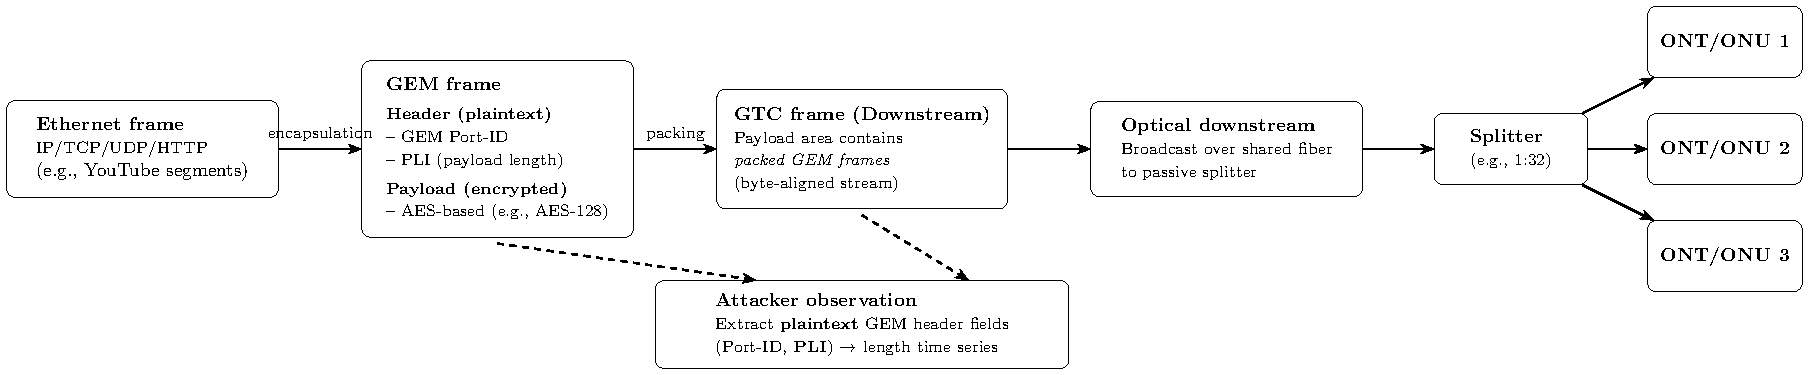
\includegraphics[width=\linewidth]{fig/gpon_encapsulation_diagram_tikz.pdf}
  \caption{Encapsulation pipeline in GPON downstream: upper-layer packets (e.g., Ethernet/IP) are encapsulated into GEM frames, packed into GTC frames, and broadcast over the shared optical line. While GEM payloads are AES encrypted (e.g., AES-128), GEM header fields such as Port-ID and PLI remain plaintext.}
  \label{fig:gpon-encapsulation}
\end{figure}

\textbf{GPON Topology and GTC Framing} GPON Networks consist of an Optical Line Terminal (OLT) at the ISP and multiple Optical Network Terminals/Units(ONTs/ONUs) (typically called "modem") deployed at subscribers. A single optical tree can serve up to 32 subscribers (e.g., 1:32 split). In the downstream, the OLT transmits downstream traffic through the splitter. Since the splitter passively distributes the optical signal from the OLT to all ONUs/ONTs on the same splitter, each ONU/ONT can physically receive the downstream transmissions destined for other ONUs/ONTs. At the transmission layer, downstream bytes are carried in GPON Transmission Convergence (GTC) frames sent periodically(per-125~$\mu$s), whose payload area carries multiple GEM frames(described next).

\textbf{GEM Framing} In GPON Network, upper layer traffic (e.g., Ethernet frames carrying TCP/IP packets) in the GEM Payload Field transmitted via GPON Encapsulation Method (GEM) Frames. Downstream GEM payloads are often encrypted for confidentiality (depending on ISP configuration~\cite{itu-g9843}). However, the GEM Port-ID (used to demultiplex services/flows) and the Payload Length Indicator (PLI), which encodes the payload size, are transmitted in plaintext. Thus, an attacker can extract a victim’s encrypted payload lengths from consecutive PLI values (optionally grouped by Port-ID), even without decrypting the payload contents.

\textbf{Video Identification} HTTP Adaptive Streaming (HAS) is the popular video streaming model -- which is generally used by video streaming platforms (e.g., Youtube, many OTT Services) --delivers video by letting the client periodically request short media segments at a bitrate chosen by an adaptive bitrate (ABR) algorithm. This request--\>response process forms characteristic bursty download patterns and bitrate-dependent segment sizes, which can be exploited for traffic inference.~\cite{bae-sec22}

\section{Threat Model}
We consider a attacker on the same optical splitter as a victim.
\begin{itemize}
  \item \textbf{1. Premise:} Attacker should have optical capture device (e.g., FPGA, modified ONU that can receive raw GTC frames) directly connecting to splitter and passively records downstream from OLT.
  *attacker does not have to get their ONU/ONT linked with OLT so if attacker remove Tx function of optic module, they can entirely record downstream records without being exposed. 
  \item \textbf{2. Collect GEMs} Then, attacker extract GTC frames from downstream traffic and they get many GEM frames. 
  \item \textbf{3. Convert GEM PLI to dataset} Then, attacker filters GEM frames corresponding to a victim's Port-ID and made a dataset containing PLI values and timestamps.
  \item \textbf{4. Dataset format} The dataset must include start & end time and duration and PLI and sequence information.
\end{itemize}
%\section{Trace Generation (125~$\mu$s)}
%To avoid relying on proprietary GPON capture hardware, we build a GPON downstream trace generator. From a PCAP of encrypted video traffic, we (i) map Ethernet frames into GEM payloads (fragmenting to satisfy the 12-bit PLI limit), (ii) generate plaintext GEM headers (PLI/Port-ID/PTI/HEC), (iii) encrypt payload bytes with AES-CTR (header remains plaintext), and (iv) pack the GEM stream into fixed-length 125~$\mu$s downstream frames consistent with the configured line rate. The attacker signal is then either the GEM-level PLI sequence or the per-frame occupancy series.
\begin{figure}[!htbp]
  \centering
  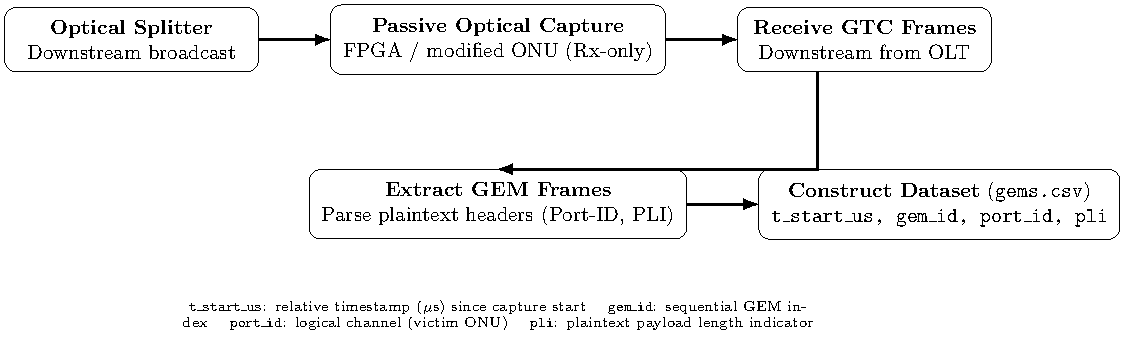
\includegraphics[width=\linewidth]{fig/attacker_pipeline_diagram_tikz.pdf}
  \caption{Attacker-side observation pipeline: passive optical capture under the same splitter enables reception of downstream GTC frames, extraction of GEM frames, and construction of a PLI-based dataset (\texttt{gems.csv}).}
  \label{fig:attacker-pipeline}
\end{figure}


\section{Experiment and Preliminary Results}
To demonstrate threat model in our experimental environment, we developed a software GPON downstream simulator that reproduces the process of receiving GTC frames, extracting GEM frames, and exporting plaintext GEM header fields into datasets. 
At first we played each of 10 videos three times in our linux based system to produce packet capture datas (PCAPs) where other streaming traffic(e.g., VNC) is restricted to minimize interference. then we simulated that PCAPs packet capture file to records the resulting PLI values and timestamps into CSV traces. 
These traces approximate the payload length observations available to a real same-splitter adversary and enable systematic evaluation of PLI-based inference.
After making dataset, we visualized cumulative PLI - Time Grapgh based on our dataset(Publicly Available on our github repository)~\cite{github}. In conclusion, We could find a clear corelation between video and cumulative PLI over time graph; Traces generated from the same video show greatly consistent slopes, which are significantly distincive to distinguish individual videos.
we assume that when adopted CNN, it is possible to distinguish video Ids using captured PLI values.
\begin{figure}[!htbp]
  \centering
  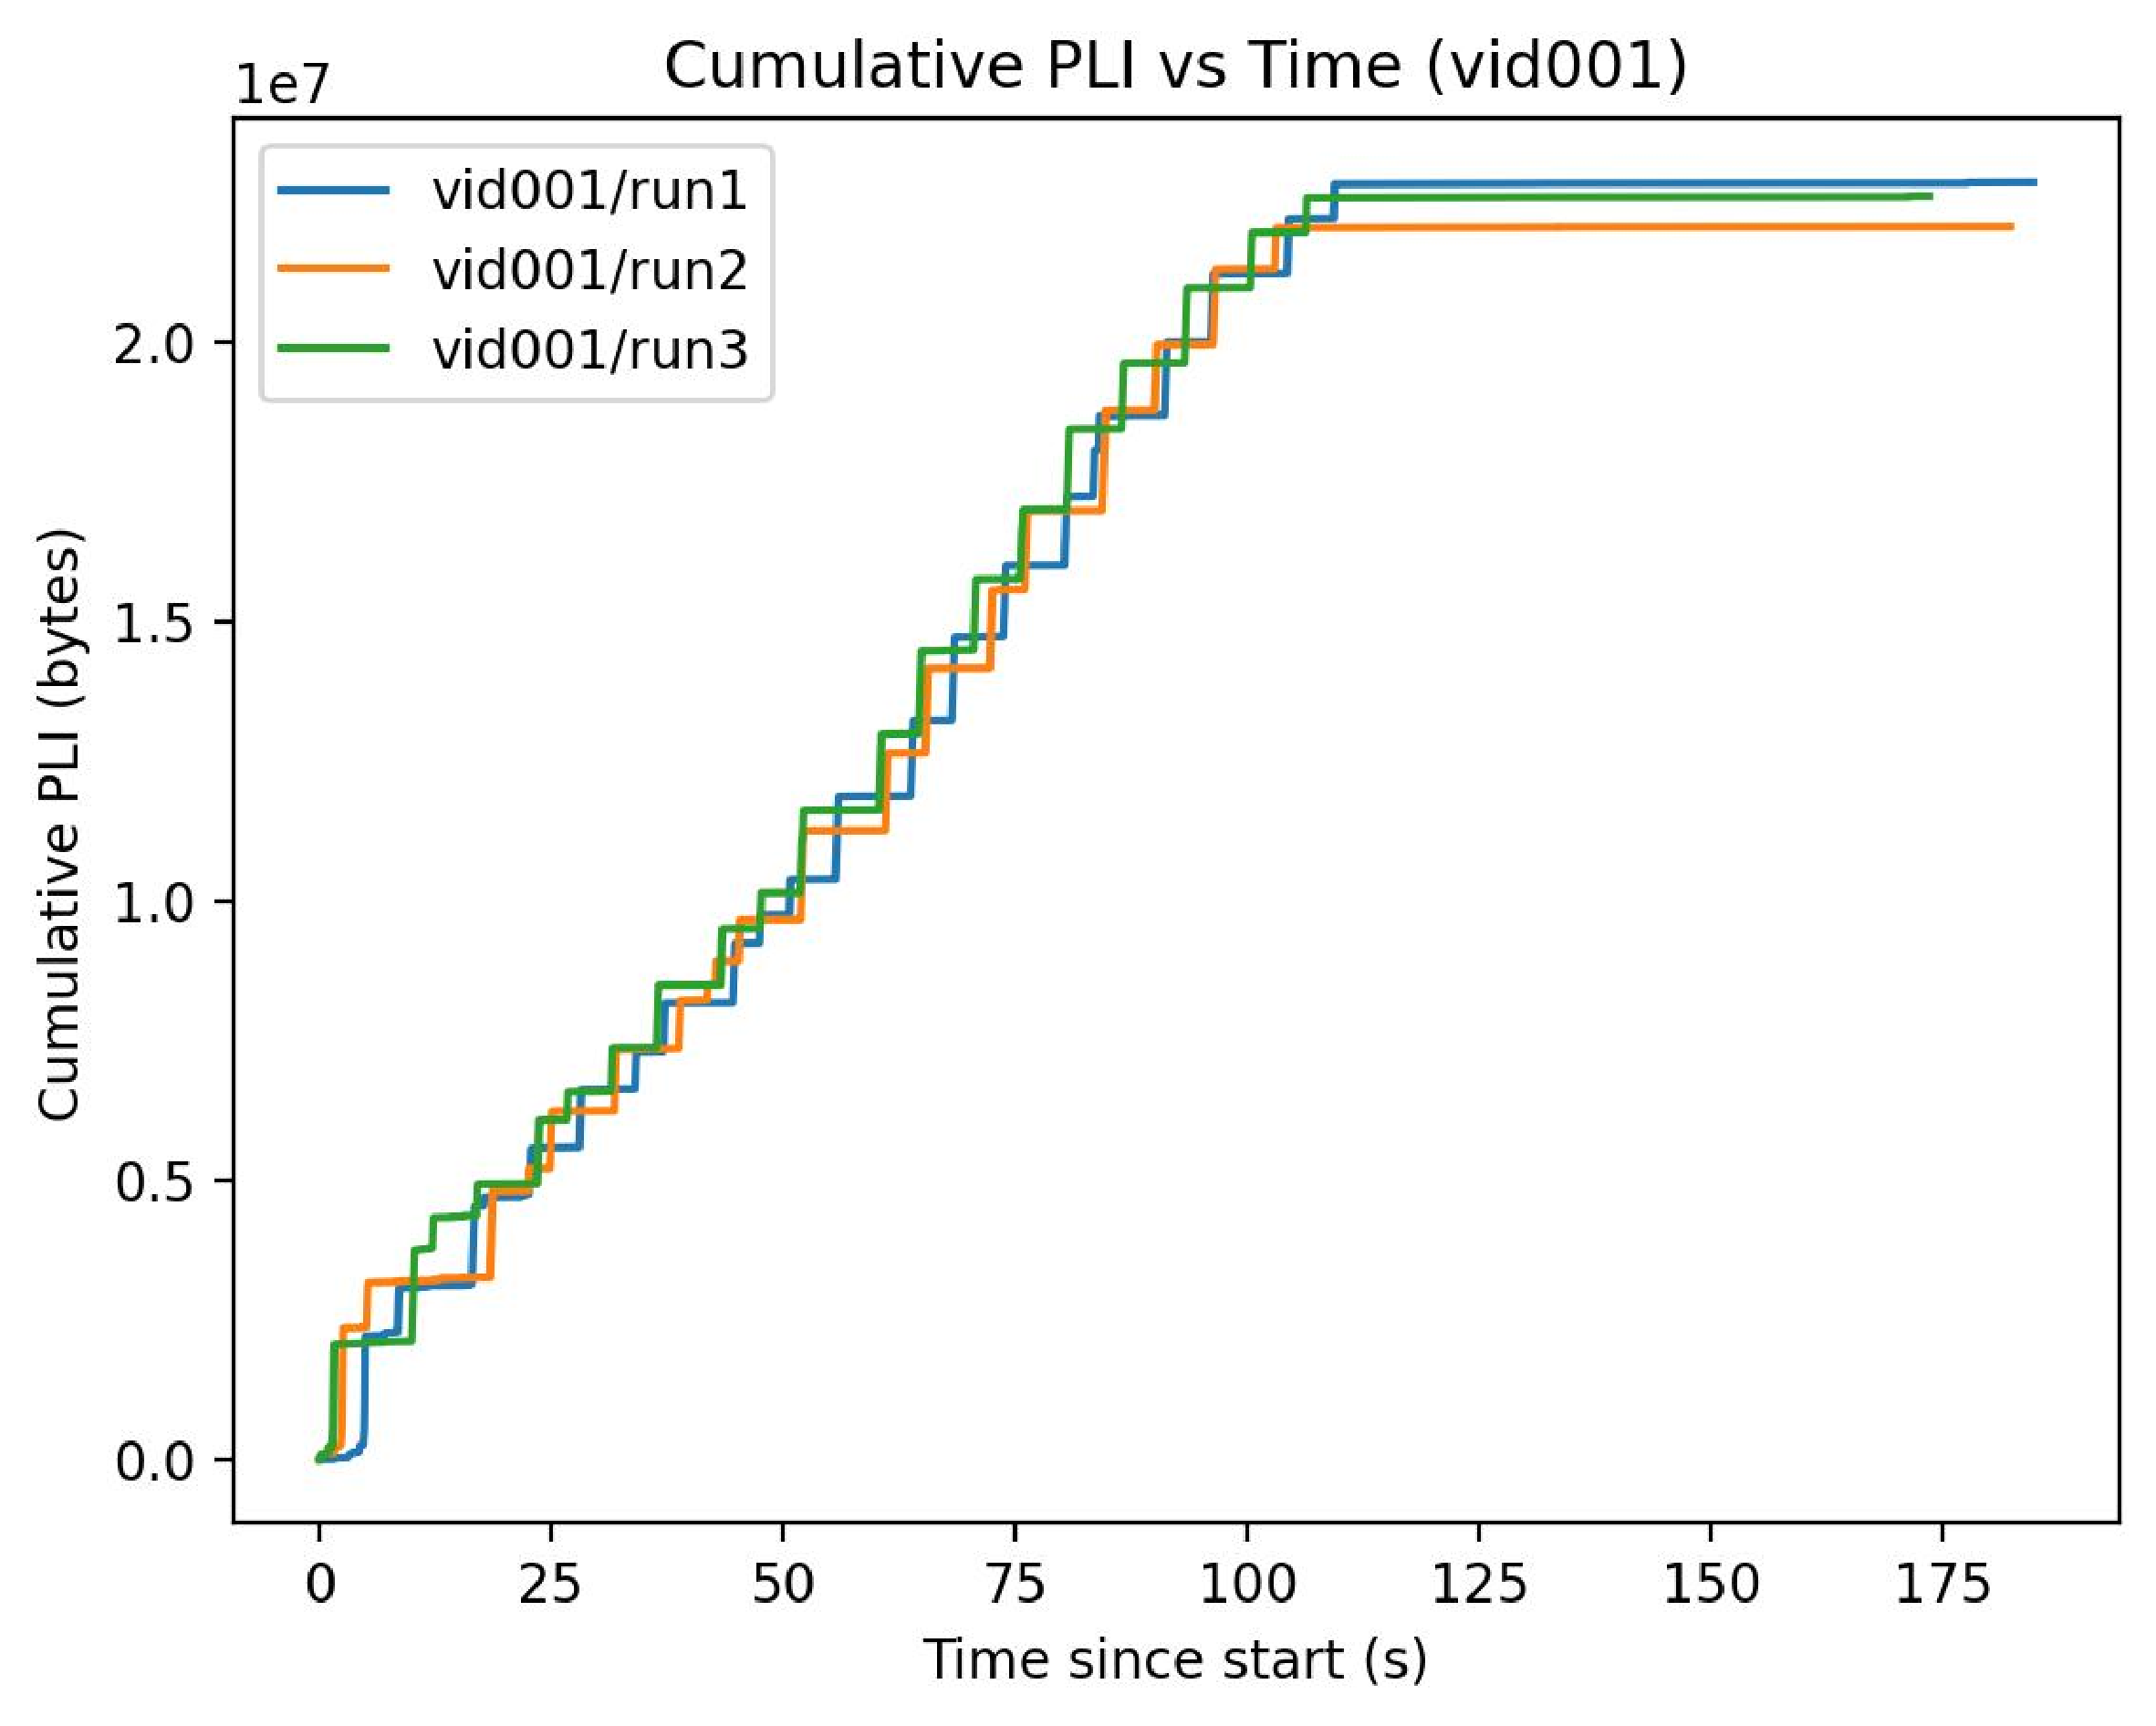
\includegraphics[width=\linewidth]{fig/cumsum_vid001.pdf}
  \caption{PLI - Time Grapgh of one of 10 videos showing that greatly identical slopes between three runs, PLI - Time Grapgh of others is publicly available on our github repository~\cite{github}.}
  \label{fig:attacker-pipeline}
\end{figure}



\section{Conclusion And Discussion}
This poster show that payload encryption in GEM is insufficient to ensure traffic confidentiality in GPON networks. 
Despite Payload Encryption, GPON Network is still vulnerable to inferring streaming activity because PLI in GEM headers can be exploited to infer a victim’s video activity(e.g., Youtube). 
Future work includes validating our observations on a real GPON testbed. 
All code and experimental dataset is publicly available on the our github repository.~\cite{github}

\textbf{Future Work In Real World.}
Future Work will be conducted in experimental testbed with Real OLT, ONU and Optical Splitter. We will use FPGA to collect GEM frames.

\textbf{Extent to XGS-PON Networks.}
Although we entirely focus on GPON in this poster, we believe that XGS-PON Networks are subject to analogous privacy risks. future work includes XGS-PON.

\textbf{Open Discussion}
We welcome open discussion on this poster. if you would like to contact us, please email us.

\section{Acknowledgment}
Note: High school student authors—please excuse any imperfect wording.
% (Conclusion and acknowledgments intentionally omitted to satisfy the 2-page poster limit.)





% trigger a \newpage just before the given reference
% number - used to balance the columns on the last page
% adjust value as needed - may need to be readjusted if
% the document is modified later
%\IEEEtriggeratref{8}
% The "triggered" command can be changed if desired:
%\IEEEtriggercmd{\enlargethispage{-5in}}

% references section

% can use a bibliography generated by BibTeX as a .bbl file
% BibTeX documentation can be easily obtained at:
% http://mirror.ctan.org/biblio/bibtex/contrib/doc/
% The IEEEtran BibTeX style support page is at:
% http://www.michaelshell.org/tex/ieeetran/bibtex/
%\bibliographystyle{IEEEtran}
% argument is your BibTeX string definitions and bibliography database(s)
%\bibliography{IEEEabrv,../bib/paper}
%
% <OR> manually copy in the resultant .bbl file
% set second argument of \begin to the number of references
% (used to reserve space for the reference number labels box)

\begin{thebibliography}{7}

\bibitem{itu-g9843}
ITU-T Recommendation G.984.3, \emph{Gigabit-capable passive optical networks (GPON): Transmission convergence layer specification}.

\bibitem{bae-sec22}
S.~Bae \emph{KAIST}, ``Watching the Watchers: Practical Video Identification Attacks in LTE Networks,'' in \emph{USENIX Security}, 2022.

\bibitem{cisco-gpon}
Cisco, ``Understand GPON Technology,'' Troubleshooting TechNotes. (Document ID: 216230) - 

\bibitem{github}
github repository - https://github.com/hjaka08/GPON

\bibitem{static}
Fiber-to-the-Home (FTTH) Market Size & Share Analysis - Growth Trends and Forecast (2025 - 2030)  - https://www.mordorintelligence.com/industry-reports/fiber-to-the-home-ftth-market

\bibitem{ytyt}
Traffic spills the beans- A robust video identification attack against YouTube - Elsevier Computers & Security (2024)

\bibitem{ytyt2}
Breaking Through the Diversity: Encrypted Video Identification Attack Based on QUIC Features - ESORICS 2024

\end{thebibliography}





% that's all folks
\end{document}


